%% This is file `elsarticle-template-1-num.tex',
%%
%% Copyright 2009 Elsevier Ltd
%%
%% This file is part of the 'Elsarticle Bundle'.
%% ---------------------------------------------
%%
%% It may be distributed under the conditions of the LaTeX Project Public
%% License, either version 1.2 of this license or (at your option) any
%% later version.  The latest version of this license is in
%%    http://www.latex-project.org/lppl.txt
%% and version 1.2 or later is part of all distributions of LaTeX
%% version 1999/12/01 or later.
%%
%% Template article for Elsevier's document class `elsarticle'
%% with numbered style bibliographic references
%%
%% $Id: elsarticle-template-1-num.tex 149 2009-10-08 05:01:15Z rishi $
%% $URL: http://lenova.river-valley.com/svn/elsbst/trunk/elsarticle-template-1-num.tex $
%%
\documentclass[preprint,12pt]{elsarticle}

%% Use the option review to obtain double line spacing
%% \documentclass[preprint,review,12pt]{elsarticle}

%% Use the options 1p,twocolumn; 3p; 3p,twocolumn; 5p; or 5p,twocolumn
%% for a journal layout:
%% \documentclass[final,1p,times]{elsarticle}
%% \documentclass[final,1p,times,twocolumn]{elsarticle}
%% \documentclass[final,3p,times]{elsarticle}
%% \documentclass[final,3p,times,twocolumn]{elsarticle}
%% \documentclass[final,5p,times]{elsarticle}
%% \documentclass[final,5p,times,twocolumn]{elsarticle}

%% The graphicx package provides the includegraphics command.
\usepackage{graphicx}
%% The amssymb package provides various useful mathematical symbols
\usepackage{amssymb}
%% The amsthm package provides extended theorem environments
%% \usepackage{amsthm}

\usepackage{algorithm}
\usepackage{algorithmic}
\usepackage{tabularx}
\usepackage{amsmath} 
\usepackage{graphicx}

%% The lineno packages adds line numbers. Start line numbering with
%% \begin{linenumbers}, end it with \end{linenumbers}. Or switch it on
%% for the whole article with \linenumbers after \end{frontmatter}.
\usepackage{lineno}

\usepackage{array}
\newcolumntype{L}[1]{>{\raggedright\let\newline\\\arraybackslash\hspace{0pt}}m{#1}}
\newcolumntype{C}[1]{>{\centering\let\newline\\\arraybackslash\hspace{0pt}}m{#1}}
\newcolumntype{R}[1]{>{\raggedleft\let\newline\\\arraybackslash\hspace{0pt}}m{#1}}

%% natbib.sty is loaded by default. However, natbib options can be
%% provided with \biboptions{...} command. Following options are
%% valid:

%%   round  -  round parentheses are used (default)
%%   square -  square brackets are used   [option]
%%   curly  -  curly braces are used      {option}
%%   angle  -  angle brackets are used    <option>
%%   semicolon  -  multiple citations separated by semi-colon
%%   colon  - same as semicolon, an earlier confusion
%%   comma  -  separated by comma
%%   numbers-  selects numerical citations
%%   super  -  numerical citations as superscripts
%%   sort   -  sorts multiple citations according to order in ref. list
%%   sort&compress   -  like sort, but also compresses numerical citations
%%   compress - compresses without sorting
%%
%% \biboptions{comma,round}

% \biboptions{}

\journal{FFT}

\begin{document}

\begin{frontmatter}

%% Title, authors and addresses

\title{\textbf{Fast Fourier Transformation}\\
\small{Design and Analysis of Algorithms}}

%% use the tnoteref command within \title for footnotes;
%% use the tnotetext command for the associated footnote;
%% use the fnref command within \author or \address for footnotes;
%% use the fntext command for the associated footnote;
%% use the corref command within \author for corresponding author footnotes;
%% use the cortext command for the associated footnote;
%% use the ead command for the email address,
%% and the form \ead[url] for the home page:
%%
%% \title{Title\tnoteref{label1}}
%% \tnotetext[label1]{}
%% \author{Name\corref{cor1}\fnref{label2}}
%% \ead{email address}
%% \ead[url]{home page}
%% \fntext[label2]{}
%% \cortext[cor1]{}
%% \address{Address\fnref{label3}}
%% \fntext[label3]{}


%% use optional labels to link authors explicitly to addresses:
%% \author[label1,label2]{<author name>}
%% \address[label1]{<address>}
%% \address[label2]{<address>}

\author{Sunil bn}

\address{University of Colorado, Boulder}

\begin{abstract}
%% Text of abstract
The fast Fourier transformations is the most important numerical algorithm in our lifetime. The FFT is used to process data throughout today's highly networked, digital world. It allows computers to efficiently calculate the different frequency components in time-varying signals-and also to reconstruct such signals from a set of frequency components. Without FFT, one wouldn't be able to login to wifi or make a call in cellphone.\\\\
This paper talks about the introduction to discrete Fourier transformations, how DFT can be computed efficiently and faster using the Cooley-Tukey algorithm. It also gives idea on how to implement FFT, detailed mathematical proof of how FFT is faster than DFT, run-time and space complexities.
\end{abstract}

\begin{keyword}
Discrete Fourier Transformation, DFT, Fast Fourier Transformation, FFT, Run-time complexity, Space complexity, Cooley-Tukey algorithm

%% keywords here, in the form: keyword \sep keyword

%% MSC codes here, in the form: \MSC code \sep code
%% or \MSC[2008] code \sep code (2000 is the default)

\end{keyword}

\end{frontmatter}

%%
%% Start line numbering here if you want
%%
%%\linenumbers

%% main text
\section{Introduction}
An algorithm for the computation of Fourier co-efficients which require less computational effort than was required in the past reported by cooley and tukey. This method was widely known as 'Fast fourier transformation'.  There are many different applications of Discrete Fourier transformations in mathematics, from simple complex number arithmetic to group theory and number theory; Therefore the efficient computation of DFT is very important. This article gives an overview of the available techniques and some of their general properties.


\section{History}
In 1805, Carl Friedrich Gauss, a German mathematician tried to determine the orbit of asteroids Pallas and Juno from sample observations. Thereby he developed discrete Fourier transformations. Unfortunately, Guass never published his work and it was lost for over one hundred years. During eighteenth century, many variations of the techniques were independently developed several times. In the early twentieth century, Carl Runge derived an algorithm similar to that of Gauss that could compute the coefficients on an input with size equal to a power of two and was later generalized to powers of three. According to Pierre Duhamel and M. Hollmann, this technique was widely known and used in the 1940's. However, after World War II, Runge's work appeared to have been forgotten for an unknown reason. Then in 1965, J. W. Cooley and J. W. Tukey published a short five page paper based on some other works of the early twentieth century which again introduced the technique which is now known as the "Fast Fourier Transform". Since the publication of Cooley-Tukey algorithm, engineer have found a number of applications for the algorithm. Over 2000 papers have been published on that topic and Fast Fourier transformations have become one of the most important techniques in the field of Electrical engineering.\\\\
Charles Fiduccia showed for the first time that the FFT can be computed in terms of algebraic modular reductions. As with the early FFT publications, this idea has been generally ignored. However, In 1942, Danielson and Lanczos published their version to compute DFT for x-ray crystallography, a field where calculation of Fourier transforms presented a formidable bottleneck. In 1965, Cooley-Tukey published a more general version of FFT which is applicable to any composite of $N$ rather than a power of 2. The below table shows the development of FFT in chronological order\cite{stefan}.

\begin{table}[ht]
\centering
\resizebox{\textwidth}{!}{\begin{tabular}{lrlrlrlrlr}
  \hline
 Researcher(s) & Date & {Length of sequence} & Number of DFT values & Applications\\ [0.5ex] 
 \hline
C.F Gauss & 1805 & Any composite integer & All & Interpolation of orbits of celestial bodies \\
F Carlini & 1828 & 12 & 7 & Harmonic analysis of barometric pressure variation \\
A. Smith & 1846 & 4, 8, 16, 32 & 5 or 6 & Correcting deviations in compasses on ship \\
J.D Everret & 1860 & 12 & 5 & Modeling underground temperature deviations \\
C. Runge & 1903 & $2^nK$ & All & Harmonic analysis of functions \\
K. Stumpff & 1939 & $2^nK$, $3^nK$ & All & Harmonic analysis of functions \\
Danielson \& Lanczos & 1942 & $2^n$ & All & X-Ray diffraction in crystals \\
L.H Thomas & 1948 & Any integer with relatively prime factors & All & Harmonic analysis of functions \\
I.J Good & 1958 & Any integer with relatively prime factors & All & Harmonic analysis of functions \\
Cooley-Tukey & 1965 & Any composite integer & All & Harmonic analysis of functions \\
S. Winograd & 1976 & Any composite integer with relatively prime factor & All & Use of complexity theory for harmonic anlaysis \\
 \hline
\end{tabular}}
\caption{Principle discoveries of Efficient Methods of Computing the DFT}
\end{table}

\section{Complex roots of unity}
In this section we will define complex roots of unity and look at some of their properties. Later we will define DFT and show how FFT computes DFT in $\Theta{(n\,log(n))}$.\\\\
A complex $nth$ root of unity is a complex number $\omega$ such that, 
$$\omega^n = 1$$
There are exactly $n$ complex $nth$ roots of unity,
$$e^{2\pi\,ik/n},\, \text{for $k = 0,1,2,...n-1$}$$
Let's use the definition of exponential of a complex number to interpret the above equation,
$$
e^{iu}=cos(u) + i\,sin(u)
$$

\begin{figure}[htbp]
    \centering
    \includegraphics [width=5cm]{Images/croots}
    \caption{$n$ complex roots of unity in complex plane}
\end{figure}

The value $\omega_n = e^{2\pi\,i/n}$ is called  the principle $n^{th}$ root of unity. The n complex nth roots of unity, 
$$\omega^0_n, \omega^1_n, \omega^2_n,...,\omega^{n-1}_n$$
form a group under multiplication. The following lemmas
furnish some essential properties of the complex nth roots of unity.\\

\subsubsection{Cancellation lemma}
\noindent
For any integer $n \ge 0$, $k \ge 0$ and $d > 0$,
$$\omega^{dk}_{dn}=\omega^{k}_{n}$$
The lemma directly follows from the equation, 
\begin{align*}
    \omega^{dk}_{dn} &=  (e^{2\pi\,i/dn})^{dk} \\
    &= (e^{2\pi\,i/n})^{k} \\
    &= \omega^k_n
\end{align*}

\subsubsection{Halving lemma}
\noindent
If $n > 0$ is even, then the squares of the n complex nth roots of unity are the n/2 complex $(n/2)$th roots of unity. \\

The lemma directly follows from the equation, 
\begin{align*}
    \omega^{dk}_{dn} &=  (e^{2\pi\,i/dn})^{dk} \\
    &= (e^{2\pi\,i/n})^{k} \\
    &= \omega^k_n
\end{align*}

\section{Discrete Fourier Transformation}
Discrete Fourier transformation converts a finite sequence of equally spaced samples of a function into the list of coefficients of a finite combination of sinusoidal, ordered by their frequencies. So DFT converts a signal from time domain to a frequency domain. In digital signal processing, the function can be sound wave signals, radio signals, temperature of a location. DFT can be implemented by numerical algorithms in computer or even in hardware.
Consider the polynomial equation,
$$A(x) = \sum_{j=0}^{n-1}a_j\,x_j$$
of degree-bound $n$ at $\omega^0_n$, $\omega^1_n$, $\omega^2_n$,...,$\omega^{n-1}_n$ (that is, at the n complex nth roots of unity).3 We assume that $A$ is given in coefficient form: $a = (a_0, a_1, ..., a_{n-1})$.Let us define the results $y_k$ , for $k=0,1,2,...,n-1$, by
\begin{align*}
    y_k &= A(\omega^k_n) \\
    &= \sum_{j=0}^{n-1}a_j\,\omega^{kj}_n
\end{align*}

The vector $y=(y_0, y_1,...,y_n)$ is the discrete fourier transform(DFT) of the coefficient vector $a=(a_0, a_1,...,a_{n-1})$. We can also write $y=DFT_n(a)$
\\\\
Given a sequence of $N$ samples $f(n)$, indexed by $n=0,1,2...N-1$, the discrete Fourier transformation is defined as $F(k)$, where $k=0,1,...N-1$.
\begin{equation*}
    F(k) = \frac{1}{\sqrt(N)}\sum_{n=0}^{n=N-1}f(n)e^{-j2\pi kn/N}
\end{equation*}

where, $F(k)$ are often called the \textit{'Fourier Coefficients'} or \textit{'Harmonics'}.

\subsubsection{DFT}
\begin{algorithm}
\caption{DFT($a$)}
\begin{algorithmic}[1]
\STATE $n \leftarrow size(a)$
\STATE $\omega_n \leftarrow cos(2\pi/n) - i\,sin\,cos(2\pi/n)$
\FOR{$k=0\,\,to\,\,n-1$}
\STATE $sum \leftarrow 0$
\FOR{$j=0\,\,to\,\,n-1$}
\STATE $sum \leftarrow sum + a[j]\cdot\,\omega_n^{kj}$
\ENDFOR
\STATE $F[k] = (1/n)\cdot sum$
\ENDFOR
\RETURN {} F
\end{algorithmic}
\end{algorithm}

\subsubsection{Discrete Fourier Transformation Analysis}
As it is evident from the above algorithm that the outer loop goes over all the $n$ samples in the signals. And for each of the iteration in the outer loop computation in the line 6 again run through all of the data points in the signal computing the product of signal value and $\omega^{n}$ raised to the power of $kj$. So the overall computation done in computing the DFT of the input vector $a$, is $\Theta{(n*n)} = \Theta{(n^2)}$.\\\\
For a DFT, $\Theta{(n^2)}$ operations are required in the computation. Whereas for an FFT only $\Theta{(n\,log(n))}$ operations are required. For example a signal with 1024 samples with straight DFT would need,
$1024^2=1048576$ operations.
For sample number of samples an FFT would require,
$1024\cdot\,log(1024) = 10240$ operations. This means that a 1024 sample FFT is 102.4 times faster than the "straight" DFT. For larger numbers of samples the speed advantage improves. For example, for 4096 samples the FFT is over 340 times faster.

\begin{figure}[htbp]
    \centering
    \includegraphics [width=7cm]{Images/dft}
    \caption{Run-time of DFT}
\end{figure}

\begin{figure}[htbp]
    \centering
    \includegraphics [width=7cm]{Images/log_dft}
    \caption{Run-time of DFT in semilogx scale}
\end{figure}

The figure[2] shows the numerical characterization of DFT along with the upper bound($c_1=.00000009$) and lower bound($c_2=.00000004$). Where the runtime of DFT is bounded by $c_1*n^2$ and $c_2*n^2$. Figure[3] shows the same plot in a semilogx scale.\\\\


\section{Fast Fourier Transformation}
A Fast Fourier transformation will compute the discrete Fourier transformation of a sequence in a efficient way. Fourier analysis converts a signal from its original domain (often time or space) to a representation in the frequency domain and vice versa. An FFT rapidly computes such transformations by factorizing the DFT matrix into a product of sparse (mostly zero) factors. FFT takes advantages of special properties of of the complex roots of unity and computes the $DFT_n(a)$ in time $\Theta{(n\,log(n))}$ as opposed to the $\Theta{(n^2)}$ time of the straightforward method.\\\\
Although strategies for dealing with non-power-of-2 sizes are known, they are beyond the scope of this book. 
The FFT method employs a divide-and-conquer strategy, using the even-indexed and odd-indexed coefficients of A(x) separately to define the two new polynomials $A^{[0]}(x)$ and $A^{[1]}(x)$ of degree-bound $n/2$:

\begin{align*}
    A^{[0]}(x) = a_0 + a_2\,x+a_4\,x^2+...+a_{n-2}x^{n/2-1} \\
    A^{[1]}(x) = a_1 + a_3\,x+a_5\,x^2+...+a_{n-2}x^{n/2-1}
\end{align*}

Note that $A^{[0]}$  contains all the even-indexed coefficients of A (the binary representation of the index ends in 0) and $A^{[1]}$ contains all the odd-indexed coefficients (the binary representation of the index ends in 1). It follows that,  
$$A(x) = A^{[0]}(x^2) + xA^{[1]}(x^2)$$
The problem of evaluating $A(x)$ at $\omega^0_n, \omega^1_n, ..., \omega^{n-1}_n$ reduces to
\begin{itemize}
    \item Evaluating the degree bound $n/2$ polynomials $A^{[0]}(x)$ and $A^{[1]}(x)$ at the points $$(\omega^0_n)^2, (\omega^1_n)^2,...,(\omega^{n-1}_n)^2$$
    and then,
    \item combining the results according to equation,\\
    By halving lemma, the list of values consists of not only $n$ distinct values but also of the $n/2$ complex $(n/2)$th roots of unity, with each root occurring exactly twice. Therefore we can evaluate recursively the polynomial $A^{[0]}$ and $A^{[1]}$ of degree-bound $n/2$ at the $n/2$ complex $(n/2)th$ roots of unity. Now these sub problems are exactly in the same form as the original problem but half the size(divide-and-conquer).  We can now divide an $n$-element $DFT_n$ computation into $n/2$-element $DFT_{n/2}$ computations.
\end{itemize}
This decomposition serves as a basis for the recursive FFT algorithm, which computes the DFT of an $n$-element vector $a=(a_0, a_1, a_2,...,a_{n-1})$, where $n$ is a power of 2.

\subsubsection{Recursive FFT}
\begin{algorithm}
\caption{Recursive-FFT($a$)}
\begin{algorithmic}[1]
\STATE $n \leftarrow size(a)$
\IF {$n=1$}
\STATE \textbf{return} a
\ENDIF
\STATE $\omega_n=e^{2\pi\,i/n}$
\STATE $\omega = 1$
\STATE $a^{[0]}=(a_0, a_2,...,a_{n-2})$
\STATE $a^{[1]}=(a_1, a_3,...,a_{n-1})$

\STATE $y^{[0]}=Recusive-FFT(a^{[0]})$
\STATE $y^{[1]}=Recusive-FFT(a^{[1]})$

\FOR{$k = 0\,\,to\,\,n/2-1$}
\STATE $y_k=y^{[0]}_k + \omega\,y^{[1]}_k$
\STATE $y^{[0]}_{k+(n/2)} = y^{[0]}_k - \omega\,y^{[1]}_k$
\STATE $\omega = \omega\,\omega_n$
\ENDFOR
\STATE \textbf{return} y
\end{algorithmic}
\end{algorithm}

\begin{figure}[htbp]
    \centering
    \includegraphics [width=7cm]{Images/treeRfft}
    \caption{Tree of input vectors to the recursive calls of the Recursive-FFT procedure. Initial invocation is for $n=8$}
\end{figure}

\subsubsection{Efficient FFT}
The practical application of DFT, such as signal processing, etc demands the utmost speed. The iterative version of FFT algorithm that that runs in $\Theta{(n\,log(n))}$ time but can have a lower constant hidden in the $\Theta$-notation than the recursive implementation of FFT. \\\\
From the recursive FFT implementation we notice that the for loop of lines 10-13 involves computing the value $\omega^k_n\,y^{[1]}_k$ twice. We can change the loop to compute it only once, storing it in a temporary variable $t$.

\begin{algorithm}
\caption{Iterative-FFT($a$)}
\begin{algorithmic}[1]
\STATE $n \leftarrow size(a)$
\IF {$n=1$}
\STATE \textbf{return} a
\ENDIF
\FOR{$k = 0\,\,to\,\,n/2-1$}
\STATE $t=\omega\,y^{[1]}_k$
\STATE $y_k = y^{[0]}_k+t$
\STATE $y_{k+(n/2)} = y^{[0]}_k-t$
\STATE $\omega = \omega\,\omega_n$
\ENDFOR
\end{algorithmic}
\end{algorithm}

The operation in the above loop, multiplying the twiddle factor $\omega = \omega^k_n$ by $y^{[1]}_k$, storing the product into $t$, and adding and subtracting $t$ from $y^{[0]}_k$, is known as \textbf{bufferfly operation} and is shown schematically in the figure below.

\begin{figure}[htbp]
    \centering
    \includegraphics [width=7cm]{Images/butterfly}
    \caption{The two input values enter from the left, the twiddle factor $\omega^k_n$ is multiplied by $y^{[1]}_k$, and the sum and difference are output on the right.}
\end{figure}

\begin{figure}[htbp]
    \centering
    \includegraphics [width=7cm]{Images/simbutterfly}
    \caption{Simplified version of butterfly operation}
\end{figure}

\subsubsection{Fast Fourier Transformation Analysis}
The recursive FFT presented above is going to work as follows: Lines 2-3 represents the base cases of the recursion. The DFT of one element is the element itself, since in this case
\begin{align*}
    y_0 &= a_0\,\omega_1^0 \\
    &= a_0\cdot\,1 \\
    &= a_0
\end{align*}
Lines 6-7 define the coefficient vector for the polynomial $A^{[0]}$ and $A^{[1]}$. Lines 4, 5 and 13 ensures that the $\omega$ is updated properly so that the whenever lines 11-12 are executed, we have $\omega = \omega^k_n$. Lines 8-9 compute the $DFT_{n/2}$ recursively, setting for $k=0,1,...,n/2-1$. 
\begin{align*}
    y^{[0]}_k = A^{[0]}\,\omega^k_{n/2}, \\
    y^{[1]}_k = A^{[1]}\,\omega^k_{n/2},
\end{align*}
or since $\omega_{n/2}^k = \omega^{2k}_n$ by cancellation lemma as mentioned previously, we get
\begin{align*}
    y^{[0]}_k = A^{[0]}\,\omega^{2k}_{n}, \\
    y^{[1]}_k = A^{[1]}\,\omega^{2k}_{n},
\end{align*}
Lines 11-12 combine the results of the recursive $DFT_{n/2}$ computations. For $y_0,y_1,...,y_{n/2-1}$, line 11 yields
\begin{align*}
    y_k &= y_k^{[0]} + \omega^k_n\,y^{[1]}_k \\
    &= A^{[0]}(\omega^{2k}_n) + \omega^{k}_n\,A^{[1]}(\omega^{2k}_n) \\
    &= A(\omega^k_n)
\end{align*}
For $y_n/2, y_{n/2+1}, ..., y_{n-1}$, letting $k=0,1,2...,n/2-1$, line 12 yields
\begin{align*}
    y_{k+n/2} &= y^{[0]}_k - \omega^k_n\,y^{[1]}_k \\
    &= y^{[0]}_k + \omega^{k+(n/2)}_{n}\,y^{[1]}_k , \text{\,\,\,\, (since $\omega^{k+(n/2)}_n = -\omega^k_n$)} \\
    &= A^{[0]}(\omega^{2k}_n) + \omega^{k+(n/2)}_n\,A^{[1]}(\omega^{2k}_n) \\
    &= A^{[0]}(\omega^{2k+n}_n) + \omega^{k+(n/2)}_n\,A^{[1]}(\omega^{2k+n}_n) \\
    &= A(\omega^{k+(n/2)}_n)  \text{\,\,\,\, (since $\omega^{2k+n}_n = \omega^{2k}_n$)} 
\end{align*}

Thus, the vector $y$ returned by the above algorithm FFT is indeed the DFT of the input vector $a$. \\\\
Lines 11 and 12 multiply each value $y_k^{[1]}$ by $\omega^k_n$, for $k=0,1,...,n/2-1$. Line 11 adds this product to $y_k^{[0]}$, and line 12 subtracts it. Because we use each factor $\omega^k_n$ in both it's positive and negative forms, we call these factors $\omega^k_n$ \textbf{twiddle factors}.\\\\
To compute the runtime of the above recursive FFT algorithm, we note that exclusive of the recursive calls, each call takes time $\Theta(n)$. Where $n$ is the length of hte input vector. This recurrence can be mathematically defined as,
\begin{align*}
    T(n) &= 2T(n/2) + \Theta{(n)} \text{\,\,\,\,(using Master's theorem)} \\
    &= \Theta{(n\,log(n))}
\end{align*}

\newpage
\subsection{Radix-2 FFT}
This algorithm is a special case of the approaches described earlier in which $n$ can be represented as a power of 2 i.e., $n = 2^k$. This means that the number of complex additions and multiplications gets reduced to $n(n+6)/2$ and $n^2/2$ just by using the divide-and- conquer approach. When we also begin to use the symmetry and periodicity property of the twiddle factor, it can be shown that the number of complex additions and multiplications can be reduced to $n\,log_2(n)$ and $(n/2)\,log_2(n)$ respectively. Hence, from a $\Theta(n^2)$ algorithm, the computational complexity has been reduced to $\Theta(n\,log(n))$.


\subsection{Radix-4 FFT}
This algorithm is similar to Radix-2 algorithm; but here, four point DFTs are performed instead of two point DFTs as in Radix-2 algorithm. This also means that the length of the input sequence, N, should be a power of 4, $4^k$. It can be shown that the number of complex multiplications and additions have been reduced to $(3n/8)log_2(n)$ and $(3n/2)log_2(n)$ respectively. Thus, it is more computationally efficient than Radix-2 FFT algorithm.

\section{Input data generation}
The input data for the fast fourier transformation in plotting the numerical characterization of runtime was generated randomly for a given $n$. The random data was generated using random module in NumPy library . 

\section{Effect of input on performance}
\subsection{Best case}
The best case is same as the average case where the input is a multiple of 2. And runtime of the FFT is $O(n\,log(n))$.

\subsection{Average case}
% There is no average case input for FFT. Any input of size greater than 1 and multiple of $2$ is going to be average case. FFT takes this input and gives a co-efficient vector of size $n$(input size). The below graphs shows the plot of input size versus runtime of DFT and FFT.
The average case input for the fast fourier transformations is when input size is a multiple of 2 i.e  $length=2^k,\ k \in \mathbb{Z}^+$. When the input is multiple of 2, the FFT make use of the symmetry to compute the fourier coefficients efficiently. The average case runtime is going to be $O(n\,log(n))$.

\subsection{Worst case}
% There is no worst case input for the FFT. Since the algorithm always divides the given input as long as it's a multiple of 2 and conquers the solution(co-efficient). 
The worst case input is same as average case and runtime is $O(n\,log(n))$.

\section{Numerical characterization of Run-time}
\subsection{Best Case}
The best case runtime of FFT is $O(n\,log(n))$ where the input size is a multiple of 2. The figure[7] shows the runtime of FFT in a unit scale which is linearithmic. The figure[8] shows the same plot of runtime vs $N$ in a semilogx scale.

\subsection{Average Case}
There is no average case input for FFT. Any input of size greater than 1 and multiple of $2$ is going to be average case. FFT takes this input and gives a co-efficient vector of size $n$(input size). The below graphs shows the plot of input size versus runtime of DFT and FFT.

\begin{figure}[htbp]
    \centering
    \includegraphics [width=7cm]{Images/fft}
    \caption{Run-time of FFT}
\end{figure}

The figure[7] shows the numerical characterization of FFT along with the upper bound($c_1=.0000003$) and lower bound($c_2=.00000019$). Where the runtime of FFT is bounded by $c_1*n\,log(n)$ and $c_2*n\,log(n)$. The figure[8] shows the same plot in semilogx scale. The figure[9] shows comparison plot of DFT and FFT.\\\\

\begin{figure}[htbp]
    \centering
    \includegraphics [width=7cm]{Images/log_fft}
    \caption{Run-time of FFT in semilogx scale}
\end{figure}

% \begin{figure}[htbp]
%     \centering
%     \includegraphics [width=7cm]{Images/test}
%     \caption{Run-time of DFT vs FFT}
% \end{figure}

\newpage
\begin{figure}[htbp]
    \centering
    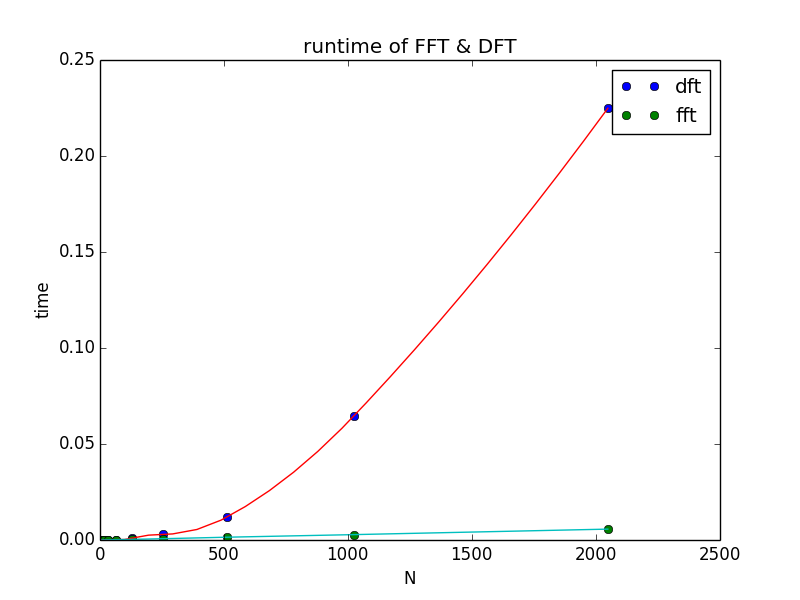
\includegraphics [width=7cm]{Images/dft_vs_fft}
    \caption{Run-time of DFT vs FFT}
\end{figure}

This graph shows the graph of DFT and FFT in a single plot. It's evident that the runtime of FFT is very very faster than the DFT with the increase in the input size.

\subsection{Worst Case}
There is no worst case input for the FFT. Since the algorithm always divides the given input as long as it's a multiple of 2 and conquers the solution(co-efficient). 

\newpage
\section{Space Complexity}
The space complexity of FFT and DFT,
\begin{itemize}
    \item The algorithm calculates the coefficients in the given input vector($n$) itself i.e in-place transformation. 
    \item The computation in FFT/DFT takes $O(1)$.
    \item The overall space complexity is going to be $O(n)$.
\end{itemize}

\section{Conclusion}
Fast Fourier transformations has many wide spread uses in scientific, engineering and mathematical applications. It has already been found that the use of the FFT methods has greatly increased the effectiveness of digital methods for a very wide range of problems such as spectral analysis, signal processing, Fourier spectroscopy, image processing, and the solution of differential equations.\\\\
Most efforts of the past several years have involved the reprogramming of previous procedures for the sake of economy in computer usage. Recent developments have been in the application of Fourier methods to problems which, due to computational effort, would not be tractable were it not for the use of the FFT method. Among these are the real-time digital Fourier methods, for which special-purpose computers are now being built. There are a number of areas in which a large amount of future development can be anticipated. Among these are the problems of the numerical solution of differential equations,image processing,and multiple time series analysis and filtering. It's used in adaptive noise cancellation filters.

\section{Future Scope}
The “communicate twice” parallel FFT algorithms are implemented such that the processors execute the butterfly operation is performed on all the inputs to the appropriate division in every stage. But that is not necessary and instead of performing computations to get the full butterfly, we can compute just half the butterfly (look at the figure 14 below) and reduce the execution time and the CPU load by half in each stage. This can be tried and benchmarked as well. \\\\The implementations that were presented in this paper were actually parallel implementations of the hugely popular and less mathematically demanding FFT algorithms. There also exist other parallel FFT algorithms that are based on matrices and Kronecker products. 
%% The Appendices part is started with the command \appendix;
%% appendix sections are then done as normal sections
%% \appendix

%% \section{}
%% \label{}

%% References
%%
%% Following citation commands can be used in the body text:
%% Usage of \cite is as follows:
%%   \cite{key}          ==>>  [#]
%%   \cite[chap. 2]{key} ==>>  [#, chap. 2]
%%   \citet{key}         ==>>  Author [#]

%% References with bibTeX database:

\section*{References}
\nocite{*}
\bibliographystyle{model1-num-names}
\bibliography{sample.bib}

%% Authors are advised to submit their bibtex database files. They are
%% requested to list a bibtex style file in the manuscript if they do
%% not want to use model1-num-names.bst.

%% References without bibTeX database:

% \begin{thebibliography}{00}

%% \bibitem must have the following form:
%%   \bibitem{key}...
%%

% \bibitem{}

% \end{thebibliography}

\end{document}

%%
%% End of file `elsarticle-template-1-num.tex'.